% Options for packages loaded elsewhere
\PassOptionsToPackage{unicode}{hyperref}
\PassOptionsToPackage{hyphens}{url}
%
\documentclass[
]{book}
\usepackage{lmodern}
\usepackage{amssymb,amsmath}
\usepackage{ifxetex,ifluatex}
\ifnum 0\ifxetex 1\fi\ifluatex 1\fi=0 % if pdftex
  \usepackage[T1]{fontenc}
  \usepackage[utf8]{inputenc}
  \usepackage{textcomp} % provide euro and other symbols
\else % if luatex or xetex
  \usepackage{unicode-math}
  \defaultfontfeatures{Scale=MatchLowercase}
  \defaultfontfeatures[\rmfamily]{Ligatures=TeX,Scale=1}
\fi
% Use upquote if available, for straight quotes in verbatim environments
\IfFileExists{upquote.sty}{\usepackage{upquote}}{}
\IfFileExists{microtype.sty}{% use microtype if available
  \usepackage[]{microtype}
  \UseMicrotypeSet[protrusion]{basicmath} % disable protrusion for tt fonts
}{}
\makeatletter
\@ifundefined{KOMAClassName}{% if non-KOMA class
  \IfFileExists{parskip.sty}{%
    \usepackage{parskip}
  }{% else
    \setlength{\parindent}{0pt}
    \setlength{\parskip}{6pt plus 2pt minus 1pt}}
}{% if KOMA class
  \KOMAoptions{parskip=half}}
\makeatother
\usepackage{xcolor}
\IfFileExists{xurl.sty}{\usepackage{xurl}}{} % add URL line breaks if available
\IfFileExists{bookmark.sty}{\usepackage{bookmark}}{\usepackage{hyperref}}
\hypersetup{
  pdftitle={R Module 1},
  pdfauthor={Alex Fout},
  hidelinks,
  pdfcreator={LaTeX via pandoc}}
\urlstyle{same} % disable monospaced font for URLs
\usepackage{color}
\usepackage{fancyvrb}
\newcommand{\VerbBar}{|}
\newcommand{\VERB}{\Verb[commandchars=\\\{\}]}
\DefineVerbatimEnvironment{Highlighting}{Verbatim}{commandchars=\\\{\}}
% Add ',fontsize=\small' for more characters per line
\usepackage{framed}
\definecolor{shadecolor}{RGB}{248,248,248}
\newenvironment{Shaded}{\begin{snugshade}}{\end{snugshade}}
\newcommand{\AlertTok}[1]{\textcolor[rgb]{0.94,0.16,0.16}{#1}}
\newcommand{\AnnotationTok}[1]{\textcolor[rgb]{0.56,0.35,0.01}{\textbf{\textit{#1}}}}
\newcommand{\AttributeTok}[1]{\textcolor[rgb]{0.77,0.63,0.00}{#1}}
\newcommand{\BaseNTok}[1]{\textcolor[rgb]{0.00,0.00,0.81}{#1}}
\newcommand{\BuiltInTok}[1]{#1}
\newcommand{\CharTok}[1]{\textcolor[rgb]{0.31,0.60,0.02}{#1}}
\newcommand{\CommentTok}[1]{\textcolor[rgb]{0.56,0.35,0.01}{\textit{#1}}}
\newcommand{\CommentVarTok}[1]{\textcolor[rgb]{0.56,0.35,0.01}{\textbf{\textit{#1}}}}
\newcommand{\ConstantTok}[1]{\textcolor[rgb]{0.00,0.00,0.00}{#1}}
\newcommand{\ControlFlowTok}[1]{\textcolor[rgb]{0.13,0.29,0.53}{\textbf{#1}}}
\newcommand{\DataTypeTok}[1]{\textcolor[rgb]{0.13,0.29,0.53}{#1}}
\newcommand{\DecValTok}[1]{\textcolor[rgb]{0.00,0.00,0.81}{#1}}
\newcommand{\DocumentationTok}[1]{\textcolor[rgb]{0.56,0.35,0.01}{\textbf{\textit{#1}}}}
\newcommand{\ErrorTok}[1]{\textcolor[rgb]{0.64,0.00,0.00}{\textbf{#1}}}
\newcommand{\ExtensionTok}[1]{#1}
\newcommand{\FloatTok}[1]{\textcolor[rgb]{0.00,0.00,0.81}{#1}}
\newcommand{\FunctionTok}[1]{\textcolor[rgb]{0.00,0.00,0.00}{#1}}
\newcommand{\ImportTok}[1]{#1}
\newcommand{\InformationTok}[1]{\textcolor[rgb]{0.56,0.35,0.01}{\textbf{\textit{#1}}}}
\newcommand{\KeywordTok}[1]{\textcolor[rgb]{0.13,0.29,0.53}{\textbf{#1}}}
\newcommand{\NormalTok}[1]{#1}
\newcommand{\OperatorTok}[1]{\textcolor[rgb]{0.81,0.36,0.00}{\textbf{#1}}}
\newcommand{\OtherTok}[1]{\textcolor[rgb]{0.56,0.35,0.01}{#1}}
\newcommand{\PreprocessorTok}[1]{\textcolor[rgb]{0.56,0.35,0.01}{\textit{#1}}}
\newcommand{\RegionMarkerTok}[1]{#1}
\newcommand{\SpecialCharTok}[1]{\textcolor[rgb]{0.00,0.00,0.00}{#1}}
\newcommand{\SpecialStringTok}[1]{\textcolor[rgb]{0.31,0.60,0.02}{#1}}
\newcommand{\StringTok}[1]{\textcolor[rgb]{0.31,0.60,0.02}{#1}}
\newcommand{\VariableTok}[1]{\textcolor[rgb]{0.00,0.00,0.00}{#1}}
\newcommand{\VerbatimStringTok}[1]{\textcolor[rgb]{0.31,0.60,0.02}{#1}}
\newcommand{\WarningTok}[1]{\textcolor[rgb]{0.56,0.35,0.01}{\textbf{\textit{#1}}}}
\usepackage{longtable,booktabs}
% Correct order of tables after \paragraph or \subparagraph
\usepackage{etoolbox}
\makeatletter
\patchcmd\longtable{\par}{\if@noskipsec\mbox{}\fi\par}{}{}
\makeatother
% Allow footnotes in longtable head/foot
\IfFileExists{footnotehyper.sty}{\usepackage{footnotehyper}}{\usepackage{footnote}}
\makesavenoteenv{longtable}
\usepackage{graphicx,grffile}
\makeatletter
\def\maxwidth{\ifdim\Gin@nat@width>\linewidth\linewidth\else\Gin@nat@width\fi}
\def\maxheight{\ifdim\Gin@nat@height>\textheight\textheight\else\Gin@nat@height\fi}
\makeatother
% Scale images if necessary, so that they will not overflow the page
% margins by default, and it is still possible to overwrite the defaults
% using explicit options in \includegraphics[width, height, ...]{}
\setkeys{Gin}{width=\maxwidth,height=\maxheight,keepaspectratio}
% Set default figure placement to htbp
\makeatletter
\def\fps@figure{htbp}
\makeatother
\setlength{\emergencystretch}{3em} % prevent overfull lines
\providecommand{\tightlist}{%
  \setlength{\itemsep}{0pt}\setlength{\parskip}{0pt}}
\setcounter{secnumdepth}{5}
\usepackage{booktabs}
% png images should be 72x72 pixels

\usepackage{xcolor}
\usepackage{colortbl}

\definecolor{bonus}{HTML}{000000}
\definecolor{reflect}{HTML}{ffcc4a}
\definecolor{assessment}{HTML}{7ea8ed}
\definecolor{progress}{HTML}{a772cc}
\definecolor{video}{HTML}{d66056}
\definecolor{caution}{HTML}{ff6700}
\definecolor{feedback}{HTML}{56cc96}

\newenvironment{bonus}
{
  \begin{center}
  \begin{tabular}{|>{\columncolor{bonus}\color{white}}p{0.9\textwidth}|}\hline\\
  
\includegraphics[scale=0.1]{src/images/sun-fill-invert.png}
  \textbf{Bonus:}
}
{\\\\\hline
  \end{tabular}
  \end{center}
}


\newenvironment{reflect}
{
  \begin{center}
  \begin{tabular}{|>{\columncolor{reflect}}p{0.9\textwidth}|}
  \hline\\
  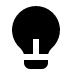
\includegraphics[scale=0.1]{src/images/lightbulb-fill.png}
  \textbf{Reflect:}
}
{\\\\\hline
  \end{tabular}
  \end{center}
}

\newenvironment{assessment}
{
  \begin{center}
  \begin{tabular}{|>{\columncolor{assessment}}p{0.9\textwidth}|}
  \hline\\
  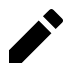
\includegraphics[scale=0.1]{src/images/pencil-fill.png}
}
{\\\\\hline
  \end{tabular}
  \end{center}
}


\newenvironment{progress}
{
  \begin{center}
  \begin{tabular}{|>{\columncolor{progress}}p{0.9\textwidth}|}
  \hline\\
  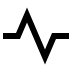
\includegraphics[scale=0.1]{src/images/pulse-line.png}
}
{\\\\\hline
  \end{tabular}
  \end{center}
}


\newenvironment{video}
{
  \begin{center}
  \begin{tabular}{|>{\columncolor{video}}p{0.9\textwidth}|}
  \hline\\
  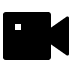
\includegraphics[scale=0.1]{src/images/vidicon-fill.png}
}
{\\\\\hline
  \end{tabular}
  \end{center}
}

\newenvironment{caution}
{
  \begin{center}
  \begin{tabular}{|>{\columncolor{caution}}p{0.9\textwidth}|}
  \hline\\
  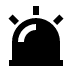
\includegraphics[scale=0.1]{src/images/alarm-warning-fill.png}
}
{\\\\\hline
  \end{tabular}
  \end{center}
}


\newenvironment{feedback}
{
  \begin{center}
  \begin{tabular}{|>{\columncolor{feedback}}p{0.9\textwidth}|}
  \hline\\
  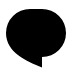
\includegraphics[scale=0.1]{src/images/chat-1-fill.png}
}
{\\\\\hline
  \end{tabular}
  \end{center}
}
\usepackage{booktabs}
\usepackage{longtable}
\usepackage{array}
\usepackage{multirow}
\usepackage{wrapfig}
\usepackage{float}
\usepackage{colortbl}
\usepackage{pdflscape}
\usepackage{tabu}
\usepackage{threeparttable}
\usepackage{threeparttablex}
\usepackage[normalem]{ulem}
\usepackage{makecell}
\usepackage{xcolor}
\usepackage[]{natbib}
\bibliographystyle{apalike}

\title{R Module 1}
\author{Alex Fout\footnote{Department of Statistics, Colorado State University, \href{mailto:fout@colostate.edu}{\nolinkurl{fout@colostate.edu}}}}
\date{2020-06-28}

\begin{document}
\maketitle

{
\setcounter{tocdepth}{1}
\tableofcontents
}
\hypertarget{welcome}{%
\chapter{Welcome!}\label{welcome}}

Hi, and welcome to the R Module 1 course at Colorado State University!

This course is the first of three 1 credit courses intended to introduce the R programming language to those with little or no programming experience.

Through these Modules (courses), we'll explore how R can be used to do the following:

\begin{enumerate}
\def\labelenumi{\arabic{enumi}.}
\tightlist
\item
  Perform basic computations and logic, just like any other programming language
\item
  Load, clean, analyze, and visualise data
\item
  Run scripts
\item
  Create reproducible reports so you can explain your work in a narrative form
\end{enumerate}

In addition, you'll also be exposed to some aspects of the broader R community, including:

\begin{enumerate}
\def\labelenumi{\arabic{enumi}.}
\tightlist
\item
  R as free, open source software
\item
  The RStudio free software
\item
  Publicly available packages which extend the capability of R
\item
  Events and community groups which advocate for the use of R and the support of R users
\end{enumerate}

More detail will be provided in the Course Topics laid out in the next chapter.

\hypertarget{how-to-navigate-this-book}{%
\subsection{How To Navigate This Book}\label{how-to-navigate-this-book}}

To move quickly to different portions of the book, click on the appropriate chapter or section in the the table of contents on the left.
The buttons at the top of the page allow you to show/hide the table of contents, search the book, change font settings, download a pdf or ebook copy of this book, or get hints on various sections of the book.
The faint left and right arrows at the sides of each page (or bottom of the page if it's narrow enough) allow you to step to the next/previous section.
Here's what they look like:

\begin{figure}

{\centering 
\includegraphics{src/images/left_arrow} 
\includegraphics{src/images/right_arrow} 

}

\caption{Left and right navigation arrows}\label{fig:unnamed-chunk-1}
\end{figure}

\hypertarget{associated-csu-course}{%
\section{Associated CSU Course}\label{associated-csu-course}}

This bookdown book is intended to accompany the associated course at Colorado State University, but the curriculum is free for anyone to access and use.
If you're reading the PDF or EPUB version of this book, you can find the ``live'' version at \url{https://csu-r.github.io/Module1/}, and all of the source files for this book can be found at \url{https://github.com/CSU-R/Module1}.

\hypertarget{prelim}{%
\chapter{Course Preliminaries}\label{prelim}}

This course is presented as a \href{https://bookdown.org/}{bookdown} document, and is divided into chapters and sections
Each week, you'll be expected to read through the chapter and complete any associated exercises, quizzes, or assignments.

\hypertarget{special-boxes}{%
\subsection{Special Boxes}\label{special-boxes}}

Throughout the book, you'll encounter special boxes, each with a special meaning.
Here is an example of each type of box:

\begin{reflect}
This box will prompt you to pause and reflect on your experience and/or
learning. No feedback will be given, but this may be graded on
completion.
\end{reflect}

\begin{assessment}
This box will signify a quiz or assignment which you will turn in for
grading, on which the instructor will provide feedback.
\end{assessment}

\begin{progress}
This box is for checking your understanding, to make sure you are ready
for what follows.
\end{progress}

\begin{video}
This box is for displaying/linking to videos in order to help illustrate
or communicate concepts.
\end{video}

\begin{caution}
This box will warn you of possible problems or pitfalls you may
encounter!
\end{caution}

\begin{bonus}
This box is to provide material going beyond the main course content, or
material which will be revisited later in more depth.
\end{bonus}

\begin{feedback}
This box will prompt for your feedback on the organization of the
course, so we can improve the material for everyone!
\end{feedback}

\hypertarget{how-this-book-displays-code}{%
\subsection{How This Book Displays Code}\label{how-this-book-displays-code}}

In addition, you may see R code either as part of a sentence like this: \texttt{1+1}, or as a separate block like so:

\begin{Shaded}
\begin{Highlighting}[]
\DecValTok{1}\OperatorTok{+}\DecValTok{1}
\end{Highlighting}
\end{Shaded}

\begin{verbatim}
[1] 2
\end{verbatim}

Sometimes (as in this example) we will also show the \textbf{output} , that is, the result of running the R code. In this case the code \texttt{1+1} produced the output \texttt{2}.
If you hover over a code block with your mouse, you will see the option to copy the code to your clipboard, like this:

\begin{figure}

{\centering 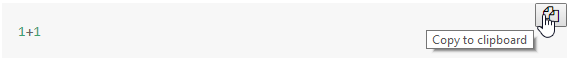
\includegraphics{src/images/copy_code} 

}

\caption{copying code from this book}\label{fig:unnamed-chunk-9}
\end{figure}

This will be useful when you are asked to run code on your computer.

\hypertarget{next-steps}{%
\subsection{Next Steps}\label{next-steps}}

When you're ready, go to the next section to learn about the course syllabus and grading policies.

\hypertarget{course-topics-syllabus}{%
\section{Course Topics \& Syllabus}\label{course-topics-syllabus}}

TODO: coming soon!

\hypertarget{schedule}{%
\subsection{Schedule}\label{schedule}}

\begin{table}[H]
\centering
\begin{tabular}{r|l|l|l|l}
\hline
Week & Weekday & Date & Reading & Assignments\\
\hline
1 & Monday & July 13 &  & \\
\hline
1 & Wednesday & July 15 &  & \\
\hline
1 & Friday & July 17 &  & \\
\hline
2 & Monday & July 20 &  & \\
\hline
2 & Wednesday & July 22 &  & \\
\hline
2 & Friday & July 24 &  & \\
\hline
3 & Monday & July 27 &  & \\
\hline
3 & Wednesday & July 29 &  & \\
\hline
3 & Friday & July 31 &  & \\
\hline
4 & Monday & August 03 &  & \\
\hline
4 & Wednesday & August 05 &  & \\
\hline
4 & Friday & August 07 &  & \\
\hline
\end{tabular}
\end{table}

\hypertarget{syllabus}{%
\subsection{Syllabus}\label{syllabus}}

\hypertarget{approach-to-learning}{%
\subsection{Approach To Learning}\label{approach-to-learning}}

\begin{itemize}
\tightlist
\item
  growth mindset
\item
  do-first
\end{itemize}

\hypertarget{grading}{%
\subsection{Grading}\label{grading}}

\hypertarget{running-your-first-r-code}{%
\section{Running your first R Code}\label{running-your-first-r-code}}

Enough of the boring stuff, let's run some R code!
Normally you will run R on your computer, but since you may not have R installed yet, let's run some R code using a website first.
As you run code, you'll see some of the things R can do.
In a browser, navigate to \href{https://rdrr.io/snippets/}{rdrr.io/snippets}, where you'll see a box that looks like this:

\begin{figure}

{\centering 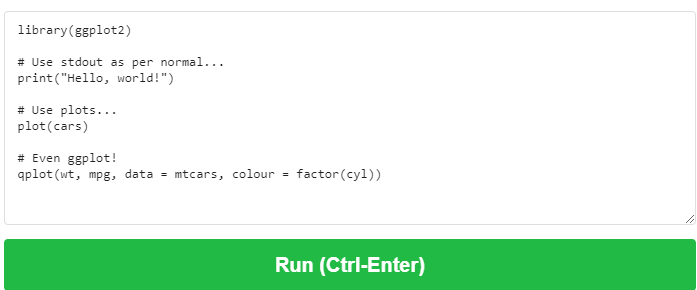
\includegraphics{src/images/rdrr} 

}

\caption{rdrr code entry box}\label{fig:unnamed-chunk-10}
\end{figure}

The box comes with some code entered already, but we want to use our own code instead, so delete all the text, starting with \texttt{library(ggplot2)} and ending with \texttt{factor(cyl))}.
In it's place, type \texttt{1+1}, then click the big green ``Run'' button.
You should see the \texttt{{[}1{]}\ 2} displayed below.
So if you give R a math expression, it will evaluate it and give the result.
Note: the ``correct answer'' to \(1+1\) is \texttt{2}, but the output also displays \texttt{{[}1{]}}, which we won't explain until later(TODO), so you can ignore that for now.

Next, delete the code you just wrote and type (or copy/paste) the following, and run it:

\begin{Shaded}
\begin{Highlighting}[]
\KeywordTok{factorial}\NormalTok{(}\DecValTok{10}\NormalTok{)}
\end{Highlighting}
\end{Shaded}

The result should be a very large number, which is equivalent to \(10!\), that is, \(10\times9\times8\times7\times6\times5\times4\times3\times2\times1\).
This is an example of an R \emph{function}, which we will discuss more in Section (TODO: insert ref).

Aside from math, R can produce plots. Try copy/pasting the following code into the website:

\begin{Shaded}
\begin{Highlighting}[]
\NormalTok{x <-}\StringTok{ }\DecValTok{-10}\OperatorTok{:}\DecValTok{10}
\KeywordTok{plot}\NormalTok{(x, x}\OperatorTok{^}\DecValTok{2}\NormalTok{)}
\end{Highlighting}
\end{Shaded}

You should see points in a scatter plot which follow a parabola.
Here's a more complicated example, which you should copy/paste into the website and run:

\begin{Shaded}
\begin{Highlighting}[]
\KeywordTok{library}\NormalTok{(ggplot2)}
\KeywordTok{theme_set}\NormalTok{(}\KeywordTok{theme_bw}\NormalTok{())}
\KeywordTok{ggplot}\NormalTok{(mtcars, }\KeywordTok{aes}\NormalTok{(}\DataTypeTok{y=}\NormalTok{mpg, }\DataTypeTok{fill=}\KeywordTok{as.factor}\NormalTok{(cyl))) }\OperatorTok{+}\StringTok{ }
\StringTok{  }\KeywordTok{geom_boxplot}\NormalTok{() }\OperatorTok{+}\StringTok{ }
\StringTok{  }\KeywordTok{labs}\NormalTok{(}\DataTypeTok{title=}\StringTok{"Engine Fuel Efficiency vs. Number of Cylinders"}\NormalTok{, }\DataTypeTok{y=}\StringTok{"MPG"}\NormalTok{, }\DataTypeTok{fill=}\StringTok{"Cylinders"}\NormalTok{) }\OperatorTok{+}\StringTok{ }
\StringTok{  }\KeywordTok{theme}\NormalTok{(}\DataTypeTok{legend.position=}\StringTok{"bottom"}\NormalTok{, }
        \DataTypeTok{axis.ticks.x =} \KeywordTok{element_blank}\NormalTok{(),}
        \DataTypeTok{axis.text.x =} \KeywordTok{element_blank}\NormalTok{())}
\end{Highlighting}
\end{Shaded}

R can be used to make many types of visualizations, which you will do more of in Section (TODO: insert ref).

\begin{bonus}
This may be the first time you've seen R, so it's okay if you don't
understand how to read this code. We'll talk more later about what each
statement is doing, but for now, here is a brief description of some of
the code above:

\begin{itemize}
\tightlist
\item
  \texttt{-10:10} This creates a sequence of numbers starting from -10
  and ending at 10. That is, \(-10, -9, -8, \ldots, 8, 9, 10\).
\item
  \texttt{library} This is a function which loads an R \emph{package}. R
  packages provide extra abilities to R.
\end{itemize}
\end{bonus}

\hypertarget{getoutoftheclass}{%
\section{What do you hope to get out of this course?}\label{getoutoftheclass}}

To close out this chapter, it would be healthy for you to reflect on what you'd like to get from this course.
Take some time to think through each question below, and write down your answers.
It is fine if your honest answer is \emph{I don't know}.
In that case, try to come up with some possible answers that \emph{might} be true.

\begin{reflect}
\begin{enumerate}
\def\labelenumi{\arabic{enumi}.}
\tightlist
\item
  Why are you taking this course?
\item
  If this course is required for your major, how do you think it is
  supposed to benefit you in your studes?
\item
  What types of data sets related to your field of study may require
  data analysis?
\item
  What skills do you hope to develop in this course, and how might they
  be applied in your major and career?
\end{enumerate}
\end{reflect}

TODO: canvas assignment?

Store your answers in a safe place, and refer to them periodically as you progress through the course.
You may find that you aren't achieving your goals and that some adjustment to how you are approaching the course may be necessary.
Or you may find that your goals have changed, which is fine!
Just update your goals so that you have something to refer back to.

\hypertarget{installingr}{%
\chapter{Installing R}\label{installingr}}

In the previous chapter, you ran R code on a website.
The purpose of this chapter is to install R on your own computer, so that you can run R without needing access to the internet.

\hypertarget{computer-basics}{%
\section{Computer Basics}\label{computer-basics}}

If you're new to computers, this section will be important for you to get set up.
If you understand the basics of operating systems, directory structures on your computer, and downloading/installing files, then you can safely skip to the next section.

\hypertarget{operating-systems}{%
\subsection{Operating Systems}\label{operating-systems}}

R works on Windows, Mac OS X, and several Linux-based operating systems, so if you have one of these operating systems, you'll be able install and use R.
At least, this is mostly true.

\begin{caution}
Some versions of Windows that run on ARM processors cannot install R,
and installing R on a Chromebook will likely be more complicated (see
\href{https://francish.netlify.app/post/installing-r-and-rstudio-on-a-pixel-slate/}{here}).
\end{caution}

\hypertarget{downloads-and-installations}{%
\subsection{Downloads and Installations}\label{downloads-and-installations}}

To install R, you'll have to download a file from the internet which performs the installation.
After you install R, you shouldn't have to download anything to run R.

TODO: take out?

\hypertarget{install-r-r-studio}{%
\section{Install R \& R Studio}\label{install-r-r-studio}}

You'll actually be installing \emph{two} separate programs, both of which are free to use.
The \emph{first} is the R programming language.
The \emph{second} is a separate program called R Studio.
R Studio will be the primary way in which you interact with R in this class, we will say more about this later.

\hypertarget{installing-r}{%
\subsection{Installing R}\label{installing-r}}

Installation will look slightly different depending on the operating system, but the major steps are the same.

\begin{itemize}
\tightlist
\item
  First, navigate to the \href{https://cran.r-project.org/mirrors.html}{CRAN Mirrors Site}, which lists several locations from which R can be downloaded.
\item
  Find a location near you (or not, this isn't critical) and click on the link to be brought to the mirror site.
\end{itemize}

From this point, this will change depending on your operating system.

\hypertarget{windows}{%
\subsubsection{Windows}\label{windows}}

\begin{itemize}
\tightlist
\item
  Click ``Download R for Windows'', then click ``base''.
\item
  Finally, Click ``Download R X.Y.Z for Windows'', where X, Y, and Z will be numbers. These numbers indicate which version of R you'll be installing. As of the publishing of this book, R is on version \texttt{r\_version}.
\item
  any other settings. Your computer might prompt for the location on your computer that you would like to save the file. Select a location (reasonable options are your Downloads folder or the Desktop) and select ``save''.
\item
  When the download completes, find the downloaded file in the File Explorer and double click to run it. This will start the installation process.
\item
  Follow the on screen prompts. For the most part you can click ``continue'', ``agree'', ``install'' as appropriate, and you don't have to worry about changing any installation settings.
\end{itemize}

\begin{video}
Create windows R install Video
\end{video}

\hypertarget{mac-os-x}{%
\subsubsection{Mac OS X}\label{mac-os-x}}

\begin{itemize}
\tightlist
\item
  Click ``Download R for (Mac) OS X''
\item
  Click ``R-X.Y.Z.pkg'', where X, Y, and Z will be numbers. These numbers indicate which version of R you'll be installing. As of the publishing of this book, R is on version \texttt{r\_version}.
\item
  Your computer might prompt for the location on your computer that you would like to save the file. Select a location and select ``save''.
\item
  When the download completes, find the downloaded file in the Finder and double click to run it. This will start the installation process.
\item
  Follow the on screen prompts. For the most part you can click ``continue'', ``agree'', ``install'' as appropriate, and you don't have to worry about changing any installation settings.
\end{itemize}

\begin{video}
?Ben? install from Mac OS X?
\end{video}

\hypertarget{installing-r-studio}{%
\subsection{Installing R Studio}\label{installing-r-studio}}

\hypertarget{successfull-installation}{%
\section{Successfull Installation}\label{successfull-installation}}

TODO: add some basic tasks here to make sure R and RStudio work. (screenshots?)

\begin{video}
todo: video orienting to R Studio (Matt video?)
\end{video}

\begin{assessment}
todo: create assessment
\end{assessment}

\hypertarget{running-code-in-rstudio-console}{%
\section{Running Code in RStudio Console}\label{running-code-in-rstudio-console}}

TODO: repeat online examples + Pull from here: \url{https://geanders.github.io/RProgrammingForResearch/r-preliminaries.html}

\begin{progress}
R comes pre-loaded with several datasets that are used in many examples.
One is a set of 150 measurements of irises from 3 species.

Use \texttt{mean(iris\$Petal.Length)} to find out what the mean petal
length is.
\end{progress}

\hypertarget{workspace-setup}{%
\section{Workspace setup}\label{workspace-setup}}

\hypertarget{recommended-settings}{%
\subsection{Recommended Settings}\label{recommended-settings}}

\begin{itemize}
\tightlist
\item
  don't save/load workspace
\item
  how to adjust font size (in options and with ctrl +/-)
\item
  dark mode!
\end{itemize}

\hypertarget{setting-working-directory}{%
\subsection{Setting working directory}\label{setting-working-directory}}

\begin{itemize}
\item
\end{itemize}

\hypertarget{create-r-studio-project-and-directories-for-class}{%
\subsection{Create R Studio Project and directories for class}\label{create-r-studio-project-and-directories-for-class}}

TODO: pull from: \url{https://geanders.github.io/RProgrammingForResearch/r-preliminaries.html\#r-scripts}

Note: This will automatically set your working directory

Folder structure:

\begin{itemize}
\item
  Raw Data
\item
  Assignments
\item
\end{itemize}

\hypertarget{reflection-assignment}{%
\section{Reflection \& Assignment}\label{reflection-assignment}}

\begin{reflect}
Before moving on to the next section, take a note of all you've done so
far.

\begin{enumerate}
\def\arabic{enumi}.{\arabic{enumi}.}
\item
  Did your R installation go smoothly? If not, could you troubleshoot
  the errors or find help online?
\item
  Does using R remind you of other programs you have experience with?
\item
  What could be some reasons that using R code written by someone else
  might not work on your computer?
\end{enumerate}
\end{reflect}

TODO: Kathleen thought this could be a progress check, I think we can have it be the first homework.

\begin{assessment}
todo: create R script to do some math, then turn in. provide template
with comment block at the top
\end{assessment}

\hypertarget{recosystem}{%
\chapter{The R Ecosystem}\label{recosystem}}

\hypertarget{the-r-programming-language}{%
\section{The R Programming Language}\label{the-r-programming-language}}

There are many important qualities to R, here are some of the most important

\hypertarget{r-is-a-programming-language}{%
\subsection{R is a Programming Language}\label{r-is-a-programming-language}}

\begin{bonus}

\end{bonus}

\hypertarget{r-is-free}{%
\subsection{R is Free}\label{r-is-free}}

\hypertarget{r-is-open-source}{%
\subsection{R is Open Source}\label{r-is-open-source}}

\hypertarget{the-r-ecosystem}{%
\section{The R Ecosystem}\label{the-r-ecosystem}}

\hypertarget{r-packages}{%
\subsection{R Packages}\label{r-packages}}

\begin{bonus}
Other notable packages
\end{bonus}

\hypertarget{r-interfaces}{%
\section{R Interfaces}\label{r-interfaces}}

\hypertarget{where-can-r-be-run}{%
\subsection{Where can R be run?}\label{where-can-r-be-run}}

\begin{video}
Video comparing the three, perhaps showing the difference between the
three.
\end{video}

\hypertarget{assignment}{%
\section{Assignment}\label{assignment}}

\begin{assessment}

\end{assessment}

\hypertarget{r-interfaces-1}{%
\subsection{R Interfaces}\label{r-interfaces-1}}

\begin{itemize}
\tightlist
\item
  RStudio
\item
  RGui
\item
  Terminal/Command line
\end{itemize}

\hypertarget{the-r-community}{%
\section{The R Community}\label{the-r-community}}

\begin{itemize}
\tightlist
\item
  Users
\item
  Package developers
\end{itemize}

Popular ``places'' that R users hang out:

Interact

TODO: need more ideas here.

Helping each other out

Where you can get help:

\begin{itemize}
\tightlist
\item
  Stack Overflow
\item
  Google!
\end{itemize}

\begin{bonus}
link to some cool visualizations, communities, etc.
\end{bonus}

\hypertarget{r-programming-fundamentals}{%
\chapter{R Programming Fundamentals}\label{r-programming-fundamentals}}

\hypertarget{programming-preliminaries}{%
\section{Programming Preliminaries}\label{programming-preliminaries}}

\begin{reflect}
\begin{reflect}

\begin{enumerate}
\def\labelenumi{\arabic{enumi}.}
\tightlist
\item
  Look at a sentence in a language you don't know, look carefully at the symbols, spacing and characters.
\item
  Recall learning a foreign language, how you had to learn the syntax and grammar rules.
\item
  Now think about English (or another language you know well) and think about the syntax and grammar rules that you take for granted.
\end{enumerate}

\end{reflect}
\end{reflect}

TODO: talk about syntax and grammar

All human languages rely on a set of rules called grammar, which describe how the language should be used to communicate.
When two humans communicate with a language, they both must agree on the the rules of that language.
R also has rules that must be followed in order for a human ( \emph{you} ) to communicate with a computer, in order to tell the computer what to do.
In human language, grammar is often fluid and evolving, and two people may have to adapt their use of the language in order to communicate.
With R, the fules are fixed, and the computer ``knows'' them perfectly.
Therefore it is up to you to learn the rules in order to make the computer do exactly what you want it to do.

Therefore it's important to cover some of the basic rules of the R programming language before you can learn all of the things R can do.
So here they are:

\hypertarget{r-commands}{%
\subsection{R Commands}\label{r-commands}}

Like most programming languages, R consists of a set of \emph{commands} which form the sequence of instructions which the computer completes. Here is an example of a command, followed by the result.

\begin{Shaded}
\begin{Highlighting}[]
\KeywordTok{print}\NormalTok{(}\StringTok{"hello, world!"}\NormalTok{)}
\end{Highlighting}
\end{Shaded}

\begin{verbatim}
[1] "hello, world!"
\end{verbatim}

This command is telling R to print out a message.
R code usually contains more than one command, and typically each command is put on a separate line.
Here are multiple commands, each on a separate line:

\begin{Shaded}
\begin{Highlighting}[]
\KeywordTok{print}\NormalTok{(}\StringTok{"The air is fine!"}\NormalTok{)}
\KeywordTok{print}\NormalTok{(}\DecValTok{1}\OperatorTok{+}\DecValTok{1}\NormalTok{)}
\KeywordTok{print}\NormalTok{(}\DecValTok{4} \OperatorTok{>}\StringTok{ }\DecValTok{5}\NormalTok{)}
\end{Highlighting}
\end{Shaded}

\begin{verbatim}
[1] "The air is fine!"
[1] 2
[1] FALSE
\end{verbatim}

The first command prints another message, the second command does some math then then prints the result, and the third command evaluates whether the statement is true or false and prints the result.
Generally, it's a good idea to put separate commands on separate lines, but you \emph{can} put multiple commands on the same line, \textbf{as long as you separate them by a semicolon}.
See this code for example:

\begin{Shaded}
\begin{Highlighting}[]
\NormalTok{x <-}\StringTok{ }\DecValTok{1}\OperatorTok{+}\DecValTok{1}\NormalTok{; }\KeywordTok{print}\NormalTok{(x); }\KeywordTok{print}\NormalTok{(x}\OperatorTok{^}\DecValTok{2}\NormalTok{)}
\end{Highlighting}
\end{Shaded}

\begin{verbatim}
[1] 2
[1] 4
\end{verbatim}

In this example, three commands are given on one line.
The first command creates a new \emph{variable} called \texttt{x}, the second command prints the value of \texttt{x}, and the third command prints the value of \texttt{x} \emph{squared}.
We see that the semicolon, \texttt{;}, serves as the command \emph{termination}, because it tells R where one command ends and another begins.
When a line contains a single command, no semicolon in necessary at the end, but including a semicolon doesn't have any effect either.

\begin{Shaded}
\begin{Highlighting}[]
\KeywordTok{print}\NormalTok{(}\StringTok{"This line doesn't have a semicolon"}\NormalTok{)}
\KeywordTok{print}\NormalTok{(}\StringTok{"This line does have a semicolon"}\NormalTok{);}
\end{Highlighting}
\end{Shaded}

\begin{verbatim}
[1] "This line doesn't have a semicolon"
[1] "This line does have a semicolon"
\end{verbatim}

\begin{caution}
Including multiple semicolons (e.g.~\texttt{print("hello");;}) does not
work!
\end{caution}

\begin{bonus}
You've just seen your first example of \emph{assignment}. That is, we
created a thing called \texttt{x} , and \emph{assigned} to it the value
of \texttt{1+1} using the \emph{assignment operator},
\texttt{\textless{}-}. Formally \texttt{x} is called an object, but
we'll talk about that more objects and assignments later.
\end{bonus}

TODO: make these code blocks display on multiple lines:

\begin{bonus}
So far, we've seen that you can place one command on one line, multiple
commands on multiple lines, multiple commands on one line, so you may
ask: can you can place one command on multiple lines? The answer is
\emph{sometimes}, depending on the command. Generally, if R is expecting
the end of a command but doesn't see one by the time it gets to the end
of a line, it will continue looking on the next line. Here are some
examples: \texttt{1\ +\ \textbackslash{}\ 1}

\texttt{print("This\ string\ is\ on\ \ multiple\ lines")}
\end{bonus}

\begin{caution}
At this point, we've introduced several new types of R commands
(assigning a variable, squaring a number, etc.), and we will talk more
specifically about these later. The important part of this section is
how R code is arranged into different \emph{commands}
\end{caution}

Lastly, commands can be ``grouped together'' using left and right curly braces: \texttt{\{} and \texttt{\}}.
Here's an example:

\begin{Shaded}
\begin{Highlighting}[]
\NormalTok{\{}
  \KeywordTok{print}\NormalTok{(}\StringTok{"here's some code that's all grouped together"}\NormalTok{)}
  \KeywordTok{print}\NormalTok{(}\DecValTok{2}\OperatorTok{^}\DecValTok{3} \OperatorTok{-}\StringTok{ }\DecValTok{7}\NormalTok{)}
\NormalTok{  w <-}\StringTok{ "hello"}
  \KeywordTok{print}\NormalTok{(w)}
\NormalTok{\}}
\end{Highlighting}
\end{Shaded}

\begin{verbatim}
[1] "here's some code that's all grouped together"
[1] 1
[1] "hello"
\end{verbatim}

The above grouped code is indented so that it looks nice, but it doesn't have to be:

\begin{Shaded}
\begin{Highlighting}[]
\NormalTok{\{}
\KeywordTok{print}\NormalTok{(}\StringTok{"here's some code that's all grouped together"}\NormalTok{)}
\KeywordTok{print}\NormalTok{(}\DecValTok{2}\OperatorTok{^}\DecValTok{3} \OperatorTok{-}\StringTok{ }\DecValTok{7}\NormalTok{)}
\NormalTok{w <-}\StringTok{ "hello"}
\KeywordTok{print}\NormalTok{(w)}
\NormalTok{\}}
\end{Highlighting}
\end{Shaded}

\begin{verbatim}
[1] "here's some code that's all grouped together"
[1] 1
[1] "hello"
\end{verbatim}

\begin{bonus}
Indenting is an example of coding \emph{style}, which are formatting
decisions which don't affect the results of the code, but are meant to
enhance readability. We'll talk more about coding style later. TODO:
talk about style later. In some programming languages, Python for
example, white space matters. That is, code indents and other spaces
change the way the code runs. In R, white space \emph{does not} matter,
so things like indents are used purely for readability.
\end{bonus}

What does it mean to ``group'' code?
At this point there is no practical difference, each command gets executed whether or not it is grouped inside curly braces.
However, code grouping will become very important later on, when we discuss \emph{control flow} in section (TODO: add ref).

\begin{progress}
In RStudio, open a new R script and type in all the R commands from this
section, to verify that you get the same result. It's good practice!
\end{progress}

\hypertarget{comments}{%
\subsection{Comments}\label{comments}}

When writing R code, you may wish to include notes which explain the code to your future self or to other humans.
This can be done with \emph{comments}, which are ignored by R when it is running the code.
The ``\#'' comment
Here's an example of some comments:

\begin{Shaded}
\begin{Highlighting}[]
\CommentTok{# Let's define y and z}
\NormalTok{y <-}\StringTok{ }\DecValTok{8}
\NormalTok{z <-}\StringTok{ }\NormalTok{y }\OperatorTok{+}\StringTok{ }\DecValTok{5} \CommentTok{# adding 5 to y and assigning the result to z}
\CommentTok{## This is still a comment, even though we're using two #'s}
\end{Highlighting}
\end{Shaded}

TODO: add note in strings section about special characters and blocks

Notice that it's possible for a line to contain only a comment, or for part of a line to be a comment.
R decides which part of a line is a comment by looking for the first ``\#'', and everything after that will be treated as a comment and ignored.

\begin{caution}
R ignores comments, but you should \emph{not}! If you're reading code
that someone else has written, it's likely that also paying attention to
their comments will greatly help you to understand what their code is
doing. It's also courteous to make good comments in your own code, if
only because you may have to return to your \emph{own} code in the
future and re-learn what it is doing! In this book, we will use comments
to help explain the R code that you will see.
\end{caution}

\hypertarget{blank-lines}{%
\subsection{Blank Lines}\label{blank-lines}}

Blank lines in R are ignored, but they can be used to organize code and enhance readability:

\begin{Shaded}
\begin{Highlighting}[]
\KeywordTok{print}\NormalTok{(}\StringTok{"The sky is blue"}\NormalTok{)}
\CommentTok{# the blank line below here is ignored}

\KeywordTok{print}\NormalTok{(}\StringTok{"The grass is green"}\NormalTok{)}
\end{Highlighting}
\end{Shaded}

\begin{verbatim}
[1] "The sky is blue"
[1] "The grass is green"
\end{verbatim}

\hypertarget{case-sensitivity}{%
\subsection{CaSe SeNsItIvItY}\label{case-sensitivity}}

In R, variables, functions, and other objects (all of which we'll talk about later), have names.
These names are case sensitive, so you must be careful when referencing an object by name.
Here we create two variables and give them different values, notice how they are different from each other:

\begin{Shaded}
\begin{Highlighting}[]
\NormalTok{A <-}\StringTok{ }\DecValTok{4}
\NormalTok{a <-}\StringTok{ }\DecValTok{5}

\KeywordTok{print}\NormalTok{(a)}
\KeywordTok{print}\NormalTok{(A)}
\end{Highlighting}
\end{Shaded}

\begin{verbatim}
[1] 5
[1] 4
\end{verbatim}

This may seem obvious, but case sensitivity applies to functions (which we'll talk about later) too.
We've been using the \texttt{print} function a lot in the above examples, which begins with a lower case p.~
There is no \texttt{Print} function:

\begin{Shaded}
\begin{Highlighting}[]
\KeywordTok{Print}\NormalTok{(}\StringTok{"testing"}\NormalTok{)}
\end{Highlighting}
\end{Shaded}

\begin{verbatim}
Error in Print("testing"): could not find function "Print"
\end{verbatim}

\hypertarget{section}{%
\subsection{?}\label{section}}

One \emph{very} nice thing in R is the documentation that accompanies it.
Every function included in R (like \texttt{print}) has documentation that explains how that function works.
To access the documentation, use a \texttt{?} followed by the name of the function, like so:

\begin{Shaded}
\begin{Highlighting}[]
\NormalTok{?print}
\end{Highlighting}
\end{Shaded}

\begin{progress}
The output of the above code chunk is not shown, because the result of
this code is best viewed in RStudio. Go to R Studio and type in
\texttt{?print} and observe what happens!
\end{progress}

\hypertarget{section-1}{%
\subsection{??}\label{section-1}}

If you don't remember the exact name of a function, or would like to search for general matches to a topic, then you can use \texttt{??}.
For example, trying \texttt{?Print} produces an error, because there is not \texttt{Print} function (remember, R is case sensitive), so there's no documentation to go with it.
However, the following should still work:

\begin{Shaded}
\begin{Highlighting}[]
\NormalTok{??Print}
\end{Highlighting}
\end{Shaded}

\begin{bonus}
Programmers have a sense of humor, too! Try running \texttt{????print}
to see a small joke. Remember, comedic taste varies!
\end{bonus}

TODO: put these bonus blocks in more appropriate places:

\begin{bonus}
\url{https://rstudio.com/wp-content/uploads/2016/10/r-cheat-sheet-3.pdf}
\end{bonus}
\begin{bonus}
Want to know more about R syntax? Try typing \texttt{?Syntax} in the R
console (then press \texttt{Enter}).
\end{bonus}

\begin{caution}
As we've seen, symbols and characters have specific meaning in R. You
must be careful not to ignore things like semicolons, curly braces,
parentheses, when reading R code. This takes practice!
\end{caution}

Okay, now that we've covered some of the basics, it's time to start learning how to do useful things in R!
The next few sections will describe the different types of data that R can handle.

\hypertarget{data-types}{%
\section{Data Types}\label{data-types}}

\begin{reflection}
TODO: what should this be?
\end{reflection}

R can store and manipulate different pieces of information, called data, and these data can be of several different types.
Here are some examples of different types of data:

\begin{Shaded}
\begin{Highlighting}[]
\NormalTok{a <-}\StringTok{ }\FloatTok{12.34}      \CommentTok{# a is a number}
\NormalTok{b <-}\StringTok{ "Hello"}    \CommentTok{# b is a string of characters}
\NormalTok{c <-}\StringTok{ }\OtherTok{TRUE}       \CommentTok{# c is a special type of data that is either true or false}
\end{Highlighting}
\end{Shaded}

R has special names for these examples, and there are other types of data as well.
Below, we'll talk about each data type, one at a time.

\begin{bonus}
The term ``data'' is actually plural! A single piece of data is called a
``datum''. So to refer to a set of data, you would say ``these data'',
and to refer to a single piece of data, you would say ``this datum''.
\end{bonus}

\hypertarget{numeric}{%
\subsection{Numeric}\label{numeric}}

Many data exist as numbers, and R has a specific data type for storing those numbers, called the \emph{numeric} data type.
Here are some examples:

\begin{Shaded}
\begin{Highlighting}[]
\NormalTok{a <-}\StringTok{ }\DecValTok{-11}
\NormalTok{b <-}\StringTok{ }\FloatTok{13.37}
\NormalTok{c <-}\StringTok{ }\DecValTok{1}\OperatorTok{/}\DecValTok{137}
\end{Highlighting}
\end{Shaded}

Note that integers, decimals, and fractions are all examples of numeric data in R.
We can prove that these are all the same data type using the \texttt{class} function:

\begin{Shaded}
\begin{Highlighting}[]
\KeywordTok{class}\NormalTok{(a)}
\end{Highlighting}
\end{Shaded}

\begin{verbatim}
[1] "numeric"
\end{verbatim}

\begin{Shaded}
\begin{Highlighting}[]
\KeywordTok{class}\NormalTok{(b)}
\end{Highlighting}
\end{Shaded}

\begin{verbatim}
[1] "numeric"
\end{verbatim}

\begin{Shaded}
\begin{Highlighting}[]
\KeywordTok{class}\NormalTok{(c)}
\end{Highlighting}
\end{Shaded}

\begin{verbatim}
[1] "numeric"
\end{verbatim}

When you have numeric data, you may want to perform math operations on them.
R has a number of built in functions to deal with numeric data, here are some examples:

\begin{Shaded}
\begin{Highlighting}[]
\KeywordTok{print}\NormalTok{(a }\OperatorTok{+}\StringTok{ }\NormalTok{b)  }\CommentTok{# Add two numeric values}
\KeywordTok{print}\NormalTok{(b }\OperatorTok{-}\StringTok{ }\NormalTok{c)  }\CommentTok{# subtract two numeric values }
\KeywordTok{print}\NormalTok{(a }\OperatorTok{*}\StringTok{ }\NormalTok{b)  }\CommentTok{# multiply two numeric values}
\KeywordTok{print}\NormalTok{(a}\OperatorTok{^}\DecValTok{3}\NormalTok{)    }\CommentTok{# take the cube of a numeric value}
\end{Highlighting}
\end{Shaded}

\begin{verbatim}
[1] 2.37
[1] 13.3627
[1] -147.07
[1] -1331
\end{verbatim}

When performing math on numeric data, R will obey \href{https://en.wikipedia.org/wiki/Order_of_operations}{order of operations}, so the following two examples will give different results:

\begin{Shaded}
\begin{Highlighting}[]
\NormalTok{a }\OperatorTok{+}\StringTok{ }\NormalTok{b }\OperatorTok{*}\StringTok{ }\NormalTok{c    }\CommentTok{# R will perform the multiplication before the addition}
\end{Highlighting}
\end{Shaded}

\begin{verbatim}
[1] -10.90241
\end{verbatim}

\begin{Shaded}
\begin{Highlighting}[]
\NormalTok{(a }\OperatorTok{+}\StringTok{ }\NormalTok{b) }\OperatorTok{*}\StringTok{ }\NormalTok{c  }\CommentTok{# R will perform the addition first, then the multiplication }
\end{Highlighting}
\end{Shaded}

\begin{verbatim}
[1] 0.01729927
\end{verbatim}

Notice that we've added extra spaces in the code to help you understand what's going on.
This is another example of code \emph{style}, which we'll talk more about later.

Notice all the decimal points?
R can be very precise when performing computations.
However, viewing all of the digits stored by R can be distracting and hard to read.
You can show just some of the digits by using the \texttt{round} function:

\begin{Shaded}
\begin{Highlighting}[]
\NormalTok{a}
\end{Highlighting}
\end{Shaded}

\begin{verbatim}
[1] -11
\end{verbatim}

\begin{Shaded}
\begin{Highlighting}[]
\KeywordTok{round}\NormalTok{(a, }\DecValTok{3}\NormalTok{)}
\end{Highlighting}
\end{Shaded}

\begin{verbatim}
[1] -11
\end{verbatim}

It also turns out that R stores \emph{more} digits than what it shows when it prints, though we won't go into detail on that now.

TODO: talk about Inf, -Inf, and NaN?

\hypertarget{integer}{%
\subsection{Integer}\label{integer}}

In general, numeric data in R are treated as if they can be any decimal number (technically, they are a \emph{double precision} number, if you know what that means).
However, there is a way to specify that a specific numeric type is an integer, by placing an ``L'' at the end of it, like so:

\begin{Shaded}
\begin{Highlighting}[]
\NormalTok{x <-}\StringTok{ }\DecValTok{20}   \CommentTok{# x will be a numeric type}
\NormalTok{y <-}\StringTok{ }\NormalTok{20L  }\CommentTok{# y will be an integer type}
\end{Highlighting}
\end{Shaded}

\begin{Shaded}
\begin{Highlighting}[]
\KeywordTok{class}\NormalTok{(x)}
\end{Highlighting}
\end{Shaded}

\begin{verbatim}
[1] "numeric"
\end{verbatim}

\begin{Shaded}
\begin{Highlighting}[]
\KeywordTok{class}\NormalTok{(y)}
\end{Highlighting}
\end{Shaded}

\begin{verbatim}
[1] "integer"
\end{verbatim}

Integers take half of the space in a computer's memory or hard drive, so if you are working with or storing a lot of numbers which are integers, it might make sense to declare them as integer type in R.
This will make more sense when we discuss vectors later.

\hypertarget{character}{%
\subsection{Character}\label{character}}

Not all data are numbers!
R also has the capability to store strings of characters, and this is the aptly named \emph{character} type (or sometimes called a \emph{character string} or just \emph{string}).
Here are some examples:

\begin{Shaded}
\begin{Highlighting}[]
\NormalTok{d <-}\StringTok{ "Hello"}         \CommentTok{# This string is defined with   *double*   quotes }
\NormalTok{e <-}\StringTok{ 'how are you?'}  \CommentTok{# This string is defined with   *single*   quotes!}
\KeywordTok{print}\NormalTok{(d)}
\KeywordTok{print}\NormalTok{(e)}
\end{Highlighting}
\end{Shaded}

\begin{verbatim}
[1] "Hello"
[1] "how are you?"
\end{verbatim}

Notice how we can define character strings using single quotes or double quotes, as long as we are consistent.
So this is not valid:

\begin{Shaded}
\begin{Highlighting}[]
\CommentTok{# Note the mismatched single/double quotes:}
\NormalTok{f <-}\StringTok{ "this does not work' }
\end{Highlighting}
\end{Shaded}

\begin{verbatim}
Error: <text>:2:6: unexpected INCOMPLETE_STRING
1: # Note the mismatched single/double quotes:
2: f <- "this does not work' 
        ^
\end{verbatim}

So, make sure you are consistent.
However, you may see another problem with this: some strings contain quotes \emph{in them}, like this:

\begin{Shaded}
\begin{Highlighting}[]
\NormalTok{g <-}\StringTok{ 'This won'}\NormalTok{t work}\StringTok{'}
\end{Highlighting}
\end{Shaded}

\begin{verbatim}
Error: <text>:1:16: unexpected symbol
1: g <- 'This won't
                   ^
\end{verbatim}

Since single quotes are being used to define the string, they can't be used in the string itself, because R will ``think'' the string is ending at the second \texttt{\textquotesingle{}}.
One option is to change the defining quotes to be double quotes, then the single quote will be safely included in the string:

\begin{Shaded}
\begin{Highlighting}[]
\NormalTok{g <-}\StringTok{ "I'm happy that this works!"}
\KeywordTok{print}\NormalTok{(g)}
\end{Highlighting}
\end{Shaded}

\begin{verbatim}
[1] "I'm happy that this works!"
\end{verbatim}

Another option is to use a backslash when using quotes inside the string, so that R ``knows'' the quote is part of the string and not ending the definition of the string:

\begin{Shaded}
\begin{Highlighting}[]
\NormalTok{g <-}\StringTok{ 'I}\CharTok{\textbackslash{}'}\StringTok{ve found another way that works!'}
\KeywordTok{print}\NormalTok{(g)}
\end{Highlighting}
\end{Shaded}

\begin{verbatim}
[1] "I've found another way that works!"
\end{verbatim}

Notice that when we define \texttt{g} we place a \texttt{\textbackslash{}\textquotesingle{}} anywhere in the string where we want a \texttt{\textquotesingle{}} to be, but when printed out, we see that R has interpreted it as just a \texttt{\textquotesingle{}}.
Notice also that we didn't have to change the defining quotes to be double quotes in this case.
The backslash is called the \emph{escape character}, and it signifies that what follows it should be interpreted \emph{literally} by R, and any special meaning should be ignored.

\begin{bonus}
Since backslash also has special meaning itself, if you want a backslash
in your string, you need to use another escape character, like so:
\texttt{g\ \textless{}-\ "here\ is\ a\ backslash:\ \textbackslash{}\textbackslash{}"}

To see a list of special characters, try typing \texttt{?Quotes} into
the R console
\end{bonus}

Here is a special string:

\begin{Shaded}
\begin{Highlighting}[]
\NormalTok{h <-}\StringTok{ ""}              \CommentTok{# This string is empty!}
\end{Highlighting}
\end{Shaded}

\texttt{h} is a character string with no characters, called an \emph{empty string}.

You can perform math on numeric data, so what can you do with strings?
The answer is, quite alot, using some functions that R provides.
Here are some of them:

\begin{Shaded}
\begin{Highlighting}[]
\KeywordTok{nchar}\NormalTok{(g)   }\CommentTok{# This prints out the number of characters in a string}
\end{Highlighting}
\end{Shaded}

\begin{verbatim}
[1] 34
\end{verbatim}

\begin{Shaded}
\begin{Highlighting}[]
\KeywordTok{substr}\NormalTok{(g, }\DecValTok{6}\NormalTok{, }\DecValTok{10}\NormalTok{)   }\CommentTok{# This extracts just part of a string, using the start and stop positions you provide}
\end{Highlighting}
\end{Shaded}

\begin{verbatim}
[1] "found"
\end{verbatim}

\begin{Shaded}
\begin{Highlighting}[]
\KeywordTok{strsplit}\NormalTok{(g, }\StringTok{" "}\NormalTok{)   }\CommentTok{# This splits the string up using a specified "delimiter" string, a single space in this case. }
\end{Highlighting}
\end{Shaded}

\begin{verbatim}
[[1]]
[1] "I've"    "found"   "another" "way"     "that"    "works!" 
\end{verbatim}

\begin{bonus}
When you split a string, this produces a \emph{list} containing a
\emph{vector} of character strings. This is an example of how data can
be organized in a structured way. We'll talk more about so called
\emph{data structures} in the next section.
\end{bonus}

\begin{Shaded}
\begin{Highlighting}[]
\KeywordTok{paste}\NormalTok{(}\StringTok{"hello"}\NormalTok{, }\StringTok{"world"}\NormalTok{)   }\CommentTok{# This combines multiple strings together into one string!}
\end{Highlighting}
\end{Shaded}

\begin{verbatim}
[1] "hello world"
\end{verbatim}

\begin{reflect}
Remember that you can learn more about a function using \texttt{?}. Type
\texttt{?paste} into R and read the documentation carefully. Can you
determine what the ``sep'' argument does? What do you think would happen
if we ran the code \texttt{print("hello",\ "world",\ sep="-")}?
\end{reflect}

There are other ways of manipulating strings, but we'll return to this later.

\hypertarget{logical}{%
\subsection{Logical}\label{logical}}

Numeric data can be any number, character types can be any string of characters, but logical data types can only be two different values: True or False
Logical data types are also known as \href{https://en.wikipedia.org/wiki/Boolean_data_type}{``boolean'' data types}.
Here we define some Logical types:

\begin{Shaded}
\begin{Highlighting}[]
\NormalTok{a <-}\StringTok{ }\OtherTok{TRUE}
\NormalTok{b <-}\StringTok{ }\OtherTok{FALSE}
\NormalTok{c <-}\StringTok{ }\NormalTok{T}
\NormalTok{d <-}\StringTok{ }\NormalTok{F}
\end{Highlighting}
\end{Shaded}

\begin{Shaded}
\begin{Highlighting}[]
\KeywordTok{print}\NormalTok{(a)}
\end{Highlighting}
\end{Shaded}

\begin{verbatim}
[1] TRUE
\end{verbatim}

\begin{Shaded}
\begin{Highlighting}[]
\KeywordTok{print}\NormalTok{(b)}
\end{Highlighting}
\end{Shaded}

\begin{verbatim}
[1] FALSE
\end{verbatim}

\begin{Shaded}
\begin{Highlighting}[]
\KeywordTok{print}\NormalTok{(c)}
\end{Highlighting}
\end{Shaded}

\begin{verbatim}
[1] TRUE
\end{verbatim}

\begin{Shaded}
\begin{Highlighting}[]
\KeywordTok{print}\NormalTok{(d)}
\end{Highlighting}
\end{Shaded}

\begin{verbatim}
[1] FALSE
\end{verbatim}

So you can see that we can define a logical type using the full name or just the first letter.
Logical data are the simplest type, but there are actually some clever things you can do with them.
You can test whether simple mathematical expressions are true or false.

\begin{Shaded}
\begin{Highlighting}[]
\CommentTok{# create x and y}
\NormalTok{x <-}\StringTok{ }\DecValTok{3}
\NormalTok{y <-}\StringTok{ }\DecValTok{4}
\CommentTok{# check: is x less than y? (should give TRUE)}
\NormalTok{x }\OperatorTok{<}\StringTok{ }\NormalTok{y}
\end{Highlighting}
\end{Shaded}

\begin{verbatim}
[1] TRUE
\end{verbatim}

The third command is a way to check if the value of \texttt{x} is less than the value of \texttt{y}.
The result of this comparison is a logical, in this case, \texttt{TRUE}.
Here are other ways of making comparisons:

\begin{Shaded}
\begin{Highlighting}[]
\NormalTok{x }\OperatorTok{<=}\StringTok{ }\NormalTok{y  }\CommentTok{# check if x is less or equal to y}
\end{Highlighting}
\end{Shaded}

\begin{verbatim}
[1] TRUE
\end{verbatim}

\begin{Shaded}
\begin{Highlighting}[]
\NormalTok{x }\OperatorTok{==}\StringTok{ }\NormalTok{y  }\CommentTok{# check if x is equal to y (note how you need two equals signs)}
\end{Highlighting}
\end{Shaded}

\begin{verbatim}
[1] FALSE
\end{verbatim}

\begin{Shaded}
\begin{Highlighting}[]
\NormalTok{x }\OperatorTok{>=}\StringTok{ }\NormalTok{y  }\CommentTok{# check if x is greater or equal to y }
\end{Highlighting}
\end{Shaded}

\begin{verbatim}
[1] FALSE
\end{verbatim}

\begin{Shaded}
\begin{Highlighting}[]
\NormalTok{x }\OperatorTok{>=}\StringTok{ }\NormalTok{y  }\CommentTok{# check if x is greater than y }
\end{Highlighting}
\end{Shaded}

\begin{verbatim}
[1] FALSE
\end{verbatim}

Comparisons can be made using strings as well:

\begin{Shaded}
\begin{Highlighting}[]
\NormalTok{x <-}\StringTok{ "Hello"}
\NormalTok{y <-}\StringTok{ "hello"}
\NormalTok{x }\OperatorTok{==}\StringTok{ }\NormalTok{y}
\end{Highlighting}
\end{Shaded}

\begin{verbatim}
[1] FALSE
\end{verbatim}

\begin{caution}
Remember that R is case sensitive, and two strings must be
\emph{exactly} the same to be considered equal.
\end{caution}

Of course any object (like \texttt{x}) will be equal to itself:

\begin{Shaded}
\begin{Highlighting}[]
\NormalTok{x }\OperatorTok{==}\StringTok{ }\NormalTok{x}
\end{Highlighting}
\end{Shaded}

\begin{verbatim}
[1] TRUE
\end{verbatim}

Surprisingly, logicals can be treated as numerics, where \texttt{TRUE} is treated as \texttt{1} and \texttt{FALSE} is treated as \texttt{0}.
Here are some examples:

\begin{Shaded}
\begin{Highlighting}[]
\OtherTok{TRUE} \OperatorTok{+}\StringTok{ }\OtherTok{TRUE}  \CommentTok{# TRUE is treated as 1}
\end{Highlighting}
\end{Shaded}

\begin{verbatim}
[1] 2
\end{verbatim}

\begin{Shaded}
\begin{Highlighting}[]
\OtherTok{FALSE} \OperatorTok{*}\StringTok{ }\DecValTok{7}  \CommentTok{# FALSE is treated as 0}
\end{Highlighting}
\end{Shaded}

\begin{verbatim}
[1] 0
\end{verbatim}

\begin{Shaded}
\begin{Highlighting}[]
\NormalTok{(}\DecValTok{2} \OperatorTok{<}\StringTok{ }\DecValTok{3}\NormalTok{) }\OperatorTok{+}\StringTok{ }\NormalTok{(}\DecValTok{1} \OperatorTok{==}\StringTok{ }\DecValTok{2}\NormalTok{)  }\CommentTok{# What's going on here? }
\end{Highlighting}
\end{Shaded}

\begin{verbatim}
[1] 1
\end{verbatim}

The last example deserves some thought. Start with each expression in parentheses, and decide whether it will evaluate to true or false.
Then remember how logicals are treated as numbers, and determine what happens when you add them together.

\begin{bonus}
\begin{bonus}

Numeric, integer, character, and logical data types are probably the most important data types to know in R, but there are others that were not covered here.
These include:

\begin{itemize}
\tightlist
\item
  complex
\item
  factor
\item
  raw
\end{itemize}

At least one of these (factor) will be covered later, but you can find more information about the other types \href{https://swcarpentry.github.io/r-novice-inflammation/13-supp-data-structures/}{here}

\end{bonus}
\end{bonus}

\begin{progress}
\begin{progress}

In the R console, type the following R commands and observe the result

\texttt{x\ \textless{}-\ "5"}

\texttt{y\ \textless{}-\ 5}

\texttt{z\ \textless{}-\ (x\ ==\ y)}

\begin{enumerate}
\def\labelenumi{\arabic{enumi}.}
\tightlist
\item
  What data type is x?
\item
  What data type is y?
\item
  What data type is z?
\item
  What is the value of z, and why does this make sense?
\end{enumerate}

\end{progress}
\end{progress}

Now that we've discussed different types of data, we'll now see how they can be structured together in meaningful ways.

\hypertarget{data-structures}{%
\section{Data Structures}\label{data-structures}}

\begin{reflection}
Imagine a grocery list, shopping list, or to-do list. That list consists
of a set of items in a specified order, and the list also has a length.
Why do you think it's useful to organize these items into a list, rather
than in some other fashion? Can you think of why it might be useful to
store data in a list?
\end{reflection}

Often, you will need to work with many data of the same type, for example:
- A sequence of measurements through time
- A grid of values
- A set of phone numbers

In these circumstances, it would make sense to organize the data into a data structure.
R provides multiple data structures, each of which are appropriate in various situations

\hypertarget{vectors}{%
\subsection{Vectors}\label{vectors}}

A vector is just an ordered set of elements (in other words, \emph{data}), all of which have the same data type.
Vectors can be created for the logical, numeric (double or integer), or character data types.
Here's an example of a vector:

\begin{Shaded}
\begin{Highlighting}[]
\NormalTok{x <-}\StringTok{ }\KeywordTok{c}\NormalTok{(}\DecValTok{1}\NormalTok{, }\DecValTok{2}\NormalTok{, }\DecValTok{3}\NormalTok{)  }\CommentTok{# this is a vector of numeric types}
\KeywordTok{print}\NormalTok{(x)}
\end{Highlighting}
\end{Shaded}

\begin{verbatim}
[1] 1 2 3
\end{verbatim}

Note that to create a vector, we use the \texttt{c} function, where c stands for \emph{combine}.
This makes sense, because we are combining three numeric objects into a numeric vector.
We may determine the length of any atomic vector like so:

\begin{Shaded}
\begin{Highlighting}[]
\KeywordTok{length}\NormalTok{(x)}
\end{Highlighting}
\end{Shaded}

\begin{verbatim}
[1] 3
\end{verbatim}

The \texttt{class} function will tell us what type of data is stored in a vector (which makes sense, because all elements of the vector have the same data type).

\begin{Shaded}
\begin{Highlighting}[]
\KeywordTok{class}\NormalTok{(x)}
\end{Highlighting}
\end{Shaded}

\begin{verbatim}
[1] "numeric"
\end{verbatim}

Here's how to create logical or numeric vectors:

\begin{Shaded}
\begin{Highlighting}[]
\NormalTok{y <-}\StringTok{ }\KeywordTok{c}\NormalTok{(}\OtherTok{TRUE}\NormalTok{, }\OtherTok{TRUE}\NormalTok{, }\OtherTok{FALSE}\NormalTok{, }\OtherTok{TRUE}\NormalTok{)}
\NormalTok{z <-}\StringTok{ }\KeywordTok{c}\NormalTok{(}\StringTok{"to"}\NormalTok{, }\StringTok{"be"}\NormalTok{, }\StringTok{"or"}\NormalTok{, }\StringTok{"not"}\NormalTok{, }\StringTok{"to"}\NormalTok{, }\StringTok{"be"}\NormalTok{) }
\end{Highlighting}
\end{Shaded}

\begin{Shaded}
\begin{Highlighting}[]
\KeywordTok{class}\NormalTok{(y)}
\end{Highlighting}
\end{Shaded}

\begin{verbatim}
[1] "logical"
\end{verbatim}

\begin{Shaded}
\begin{Highlighting}[]
\KeywordTok{length}\NormalTok{(y)}
\end{Highlighting}
\end{Shaded}

\begin{verbatim}
[1] 4
\end{verbatim}

\begin{Shaded}
\begin{Highlighting}[]
\KeywordTok{class}\NormalTok{(z)}
\end{Highlighting}
\end{Shaded}

\begin{verbatim}
[1] "character"
\end{verbatim}

\begin{Shaded}
\begin{Highlighting}[]
\KeywordTok{length}\NormalTok{(z)}
\end{Highlighting}
\end{Shaded}

\begin{verbatim}
[1] 6
\end{verbatim}

\begin{reflect}
\begin{reflect}

The above statement states that all elements of a vector must have the same data type, so what do you think will happen if you try to create a vector using elements from different data types?
Here are some possibilities, can you think of another one?

\begin{itemize}
\tightlist
\item
  R will produce an error
\item
  R will combine the elements somehow, but the result won't be a vector
\item
  Something else?
\end{itemize}

Whatever happens, humans were behind the decision of how R should behave in this situation.
If you were in charge of making this decision, what would make the most sense?

\end{reflect}
\end{reflect}
\begin{progress}
Let's try to create a vector of mixed type and see what happens. Run the
following commands in R and think about the output:

\texttt{m\ \textless{}-\ c(TRUE,\ "Hello",\ 5)}

\texttt{class(m)}

\texttt{print(m)}

What changes did R make when creating the vector?
\end{progress}

```

\hypertarget{another-data-type-factors}{%
\subsection{Another Data Type? Factors}\label{another-data-type-factors}}

\hypertarget{practice}{%
\section{Practice}\label{practice}}

\begin{progress}
asdf
\end{progress}

\hypertarget{r-objects}{%
\section{R Objects}\label{r-objects}}

\hypertarget{everything-is-an-object-in-r}{%
\subsection{\texorpdfstring{\emph{Everything} is an object in R}{Everything is an object in R}}\label{everything-is-an-object-in-r}}

\hypertarget{assigning-objects}{%
\subsection{Assigning Objects}\label{assigning-objects}}

\begin{bonus}
asdf
\end{bonus}

\hypertarget{inspecting-objects}{%
\subsection{Inspecting objects}\label{inspecting-objects}}

str, names, dim

\hypertarget{null-objects}{%
\subsection{Null Objects}\label{null-objects}}

\hypertarget{quiz}{%
\section{Quiz}\label{quiz}}

\begin{assessment}
asdf
\end{assessment}

\hypertarget{loading-saving-data}{%
\section{Loading / Saving Data}\label{loading-saving-data}}

\hypertarget{taster-list-of-file-forms-and-sources}{%
\subsection{``Taster''(?) list of file forms and sources}\label{taster-list-of-file-forms-and-sources}}

\hypertarget{readingwriting-csv}{%
\subsection{reading/writing csv}\label{readingwriting-csv}}

\hypertarget{best-practices}{%
\subsection{Best practices}\label{best-practices}}

principles of Tidy Data (wickham 2014)

raw data as read only

\hypertarget{downloading-and-saving}{%
\section{Downloading and Saving}\label{downloading-and-saving}}

\begin{video}
downloading and saving example csv from canvas or website
\end{video}

\hypertarget{working-with-data}{%
\section{Working With Data}\label{working-with-data}}

\hypertarget{summarizing-vectors}{%
\subsection{Summarizing vectors}\label{summarizing-vectors}}

Mean, std, etc.

\hypertarget{summarizing-matrices}{%
\subsection{Summarizing matrices}\label{summarizing-matrices}}

\hypertarget{summarizing-vectors-1}{%
\subsection{Summarizing vectors}\label{summarizing-vectors-1}}

\hypertarget{basic-plotting}{%
\subsection{Basic Plotting}\label{basic-plotting}}

\begin{bonus}
ggplot example
\end{bonus}

\hypertarget{basic-indexing}{%
\subsection{Basic indexing}\label{basic-indexing}}

\hypertarget{advanced-indexing}{%
\subsection{Advanced indexing}\label{advanced-indexing}}

\begin{bonus}
dplyr example
\end{bonus}

\hypertarget{practice-1}{%
\section{Practice}\label{practice-1}}

\begin{progress}
asdf
\end{progress}

\hypertarget{basic-control-flow}{%
\section{Basic Control Flow}\label{basic-control-flow}}

If/else

loops (for, while)

switch

\hypertarget{advanced-control-flow}{%
\section{Advanced Control Flow}\label{advanced-control-flow}}

*apply family

\hypertarget{writing-functions}{%
\section{Writing FUnctions}\label{writing-functions}}

Function scope

\begin{bonus}
\begin{itemize}
\tightlist
\item
  Pass by value, contrast with other languages
\end{itemize}
\end{bonus}

\hypertarget{working-with-popular-packages}{%
\section{Working With Popular Packages}\label{working-with-popular-packages}}

\hypertarget{assignment-1}{%
\section{Assignment}\label{assignment-1}}

\begin{assessment}
Make R Markdown PDF that covers most/all of CH4: read in data, do basic
things with it.
\end{assessment}

  \bibliography{src/book.bib}

\end{document}
